\section{Authoring Tools for XR}
\label{sec:background-authoring}
In the following chapter an exhaustive background of the thesis research field is provided for a better understanding of the research work and the related works in this topic. The chapter starts with \autoref{sec:ar-authoring} entering into the details of the AR authoring tools and their categorization. Later, we presents a literature review of AR authoring tools divided into programming tools and content design tools, with an emphasis on the immersive ones. The next \autoref{subsec:vr-authoring}, on the other hand, provides an overview of authoring tools in VR followed by the related works found in the literature. 

\subsection{AR Authoring}
\label{sec:ar-authoring}
The continuous growth of consumer electronics such as smartphones and their computational power has led to an increasing interest in AR applications, thanks to their ability to engage the users.
However the process to create an AR application requires a long and time-consuming pipeline, involving expertise in different areas such as computer science and 2D/3D graphic design. The latter is especially needed when dealing with complex and accurate 3D models, which can be modeled with Computer-Aided Design (CAD) tools (e.g. AutoCAD\footnote{https://www.autodesk.com/products/autocad/overview}, SolidWorks\footnote{https://www.solidworks.com}) and then converted using a DCC software (e.g. Blender\footnote{https://www.blender.org}) in a suitable file format for AR engines \cite{de_paolis_waat_2020}.

To facilitate and speed up the development of AR experiences several authoring tools have been proposed and commercialized: the authoring tools can be categorized into programming tools and content design tools \cite{marcus_authoring_2016}. While the former tools represent IDEs, frameworks or high-level APIs, the latter add various levels of abstractions reducing or, in some cases, removing the programming capability given their content driven nature.
In their work, Roberto et al.~\cite{marcus_authoring_2016} also provide a further classification of these tools depending on the level of application interface abstraction and concept abstraction, as seen in \autoref{fig:authoring-tools}.
\begin{figure}[h]
	\centering
	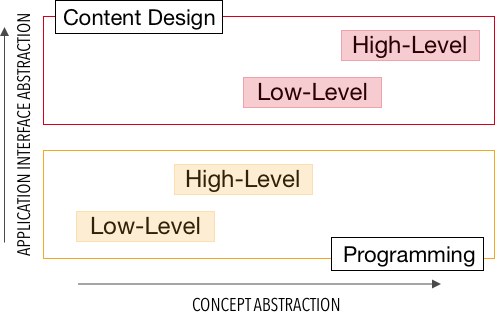
\includegraphics[width=8.5cm]{Background/authoring-tools.png}
	\caption{Categorization of AR authoring tools \cite{marcus_authoring_2016}.}
	\label{fig:authoring-tools}
\end{figure}
The two categories described above are organized into low-level and high-level. Programming tools are distinguished among those ones using low-level coding (i.e. requiring access to system primitives) and those working with high-level libraries.
Increasing the abstraction level of these tools we find the low-level content design tools, that require some scripting skills to add behaviors to AR contents and the high level content design tools, also known as \glspl{HCDF}, that abstract from the coding layer through a visual programming logic. This allows non-programmers to focus more on the interactions and behaviors of objects than their renderings.

Another classification of authoring tools is provided by Nebeling and Speicher \cite{nebeling_trouble_2018}, without a specific focus on AR experiences but instead considering both AR and VR applications. They based their classification on the level of design fidelity achieved using a specific tool and the skills and resources required by the users to use it.

Apaza et al.~\cite{apaza_systematic_2018} focused their investigation in \glspl{HCDF} through a systematic mapping and analysis of the current trends in the context of this development approach. 
They found that, after a first period dominated by the PC where the most common user interfaces were 2D and Non-immersive 3D, the development platform have been moving to different platforms as the web, \gls{HHD} and \gls{HMD}, with an increasing interest into immersive 3D user interfaces. The authors consider the authoring tools with an immersive 3D UI a “hot topic” given their WYSIWYG nature of editors.

\subsubsection{Development and Deployment Paradigms}
In \cite{marcus_authoring_2016} is described an analysis on the authoring and deployment paradigms of AR authoring tools. Two approaches characterize the authoring process: Stand-Alone and AR Plug-In.
The \textbf{Stand-Alone} approach is adopted by authoring solutions that include all the components required for a complete development of AR applications, as a GUI, rendering engines, and tracking options. The \textbf{AR Plug-In} paradigm uses, instead, a third-party component acting as plugin for a target software that, natively, would not support AR authoring. This components usually consist of GUI elements to configure a desired experience.

The last important step at the end of the authoring process is the deployment, consisting in two different strategies: the Platform-Specific and Platform-Independent methods. A \textbf{Platform-Specific} (PS) deployment compiles the AR project in as many software packages as the number of deployment targets, being these native applications for a specific OS and, sometimes, hardware. 
The most interesting approach is, undoubtedly, the \textbf{Platform-Independent} (PI) deployment. It allows to export each AR experience in data files to be read on an AR browser acting as software platform (SP) running on the end-user device with the advantage that only one app is needed for multiple contents. A commercial example is given by Layar\footnote{https://layar.com}.

\subsubsection{Related Works}
\label{sec:related-works}
Over the years, several authoring software and programming environments have emerged in the field of AR applications development. This section gives an understanding of these tools, divided by their abstraction level (\autoref{fig:authoring-tools}, with a particular focus on Content Design Tools and their sub-branch of Immersive Content Design Tools.
\subsubsection{Programming Tools}
\label{subsec:related-programming-tools}
AR authoring programming tools can consist of IDEs, libraries or frameworks and are usually used in combination with other tools to boost the authoring process.
These libraries are usually written in a low-level programming language like C/C++, therefore they require the user to have a specific programming knowledge. These libraries, of which ARToolkit\footnote{http://www.artoolkitx.org} \cite{kato1999marker} is one of the first examples, require the user to worry about low-level tasks such as marker tracking, spacial mapping or objects rendering \cite{stephanidis_authoring_2020},  while their high-level counterparts allow users to only code the interaction techniques or visualization of objects \cite{stephanidis_authoring_2020}.

Unity\footnote{https://unity.com} is an example of high-level programming tool, it is a professional game development environment that allows to visualize and manipulate simulations of AR scenes, moving geometries into them and editing their appearance. However, to author interactions, Unity requires coding through the C\# programming language and the AR functionalities are added by the Vuforia SDK\footnote{https://www.ptc.com/en/products/vuforia}, supporting features like tracking and visualization of contents.

\subsubsection{Content Design Tools}
\label{subsec:related-content-design-tools}
Content design tools require little to zero knowledge of programming in favor of a GUI that allows interactions and content authoring. Although very easy for rapid prototyping of AR applications, they may limit the customization of the designed experience achieved through programming tools.

DART (Designer's AR Toolkit), a plugin for Adobe Director now out of commerce, is an example of the earliest low-level content design tools. It was intended for multimedia designers to test AR designs and turn storyboards into minimum viable products by adding behaviors to objects either by dragging and dropping or by writing scripts using the Lingo scripting language. Wikitude Studio\footnote{https://www.wikitude.com/products/studio/} allows to create AR contents to be exported and read by the Wikitude AR browser app with a simple drag and drop interface of the editor and its workflow; Amazon Sumerian\footnote{https://aws.amazon.com/sumerian/}, instead, can be used to build quick AR web experiences accessible by mobile browsers on AR-enabled devices starting from .fbx 3D models to be added into the scene view.

HoloBuilder \cite{nebeling_trouble_2018} (\autoref{fig:holobuilder}) is a high-level tool defined by the authors as “a PowerPoint for AR applications”; it enables everyone to design experiences based on custom images or point clouds\footnote{https://en.wikipedia.org/wiki/Point\_cloud} as markers and the changes of states of the app is represented by the change of different “slides”. The authors also highlight several problems of HoloBuilder which are exploited to design a better tool, as the two proposed in their paper: ProtoAR and GestureWiz, both inspired by DART. Another similar tool is described in Villanueva et al.~\cite{villanueva_meta-ar-app_2020}, in which an authoring software for educators shows a canvas in which object animations can be created by choosing two points of the path that is automatically computed, while both QR code tracking and ground detection augmentation methods are supported.

\begin{figure}[h]
    \centering
    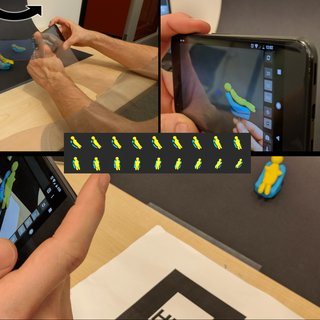
\includegraphics[width=0.5\textwidth]{Figures/Background/tools/Holobuilder.jpg}
    \caption{Content Design Tool Examples - HoloBuilder}
    \label{fig:holobuilder}
\end{figure}

SimpleAR has been defined as the \gls{HCDF} aimed at users with no programming knowledge \cite{apaza-yllachura_simplear_2019} and it can be adapted to any AR programming framework given its framework abstraction. Indeed, end users can easily create mobile AR apps by calling primitive methods as obtaining a 3D model or triggering change of states after events by building the application logic through a visual programming editor in Google Blockly\footnote{https://developers.google.com/blockly/} as web app. A viewer, finally, shows the AR application modeled in the editor, reading the configuration from a Firebase database and downloading the 3D models through Google Poly\footnote{https://blog.google/products/google-ar-vr/poly-browse-discover-and-download-3d-objects-and-scenes/} APIs.

Another example of low-level content design tool is given by Lécuyer et al.~\cite{lecuyer_authoring_2019}, in which the proposed authoring tool exploits and adopts the object-relation paradigm already known in VR development, dividing the tool in a designer's part for the content authoring and a developer's part to implement the interactions. The created content is exported in a Unity project containing data about the scene, the interactions and tracking information, to allow a separation of concerns in favor of code re-usability.
Kurt et al.~\cite{kurt_argent_2020} analyze the processes involved in AR application development and, in their work, propose a pipeline of standardized processes called ARgent framework. The workflow steps consist of \textit{Uploading Assets}, \textit{Importing Assets}, \textit{Creating Animations}, \textit{Scripting} and \textit{AR-based Application testing}. The architecture of  this framework consists of a web interface written in HTML and JavaScript communicating with a WebServer connected to the database, this is used for assets management while scripting capabilities are achieved through the JavaScript programming language; eventually, the testing process allows the designer to experience the AR scene created, using methods as marker tracing or ground plane tracking.

A peculiar yet interesting way to design AR experiences is proposed and implemented in the work by Shekhar et al.~\cite{shekhar_arcomposer_2019}: ARComposer (\autoref{fig:shekhar}), indeed, is a mobile application that leverages the advances in machine learning text analysis techniques to provide an interface where the authoring of AR scenes is entirely described by text; spacial arrangements are predicted as well as additional common objects are added based on common-world knowledge, and it supports both static and dynamic scenes.

\begin{figure}[h]
    \centering
    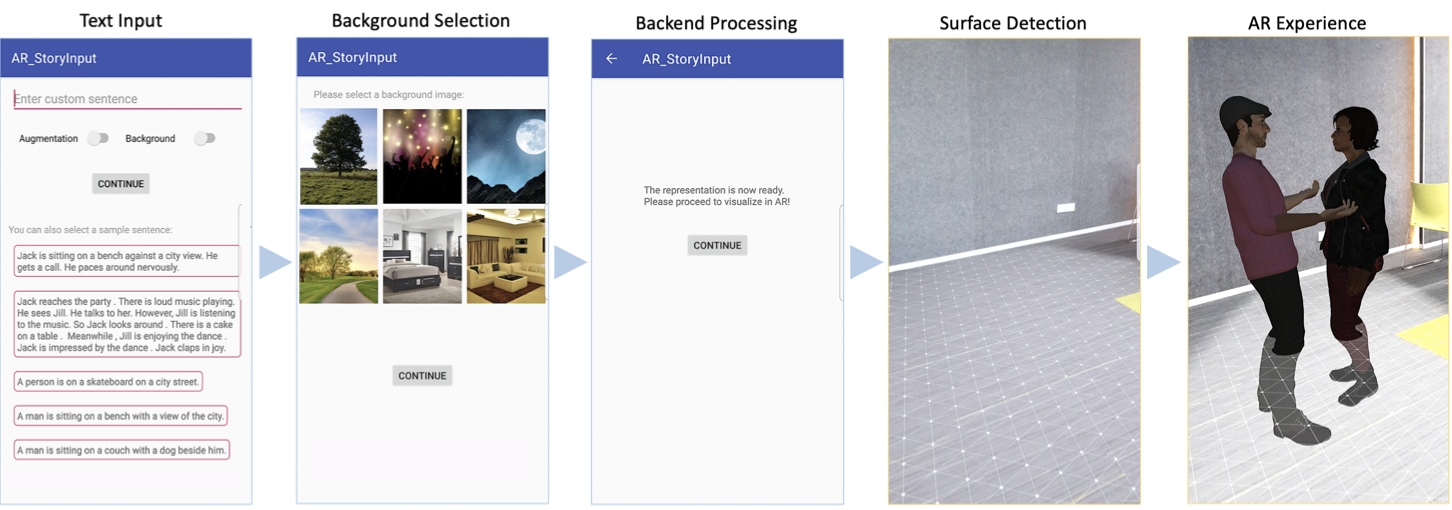
\includegraphics[width=\textwidth]{Figures/Background/tools/Shekhar.png}
    \caption{Content Design Tool Examples - ARComposer}
    \label{fig:shekhar}
\end{figure}

\subsubsection{Immersive Content Design Tools}
\label{subsec:related-immersice-hcdf}
3D GUI authoring tools are examples of immersive authoring tools, proposed by Lee et al.~\cite{lee2005immersive}, in which objects' behaviors and interactions are defined within the same AR interface that shows them. They are usually deployed on \gls{HMD} devices but in some cases \glspl{HHD} are also a good alternative, allowing in-situ authoring of experiences and direct manipulation of 3D objects.

Yang et al.~\cite{yang_interactive_2016} provide one of the first examples, an AR development environment without programming, where contents are directly rendered by a \gls{HMD} and user inputs are registered through a mobile device, that provides audio and haptic feedback. CAVE-AR \cite{cavallo_cave-ar_2019} (\autoref{fig:cavallo}), instead, uses VR to simulate the AR environment in which the experience is designed, independently of users' devices, blending the coordinate system of the two environments, mixing geographical information, architectural details and sensor data to debug the context of a typical AR use case scenario.

\begin{figure}[h]
    \centering
    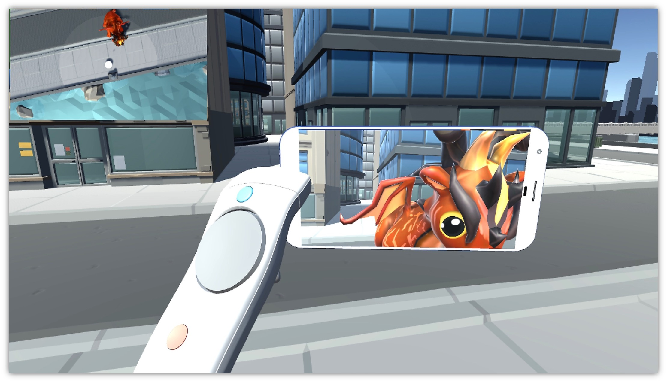
\includegraphics[width=0.75\textwidth]{Figures/Background/tools/cavallo.png}
    \caption{Content Design Tool Examples - CAVE-AR}
    \label{fig:cavallo}
\end{figure}

WAAT\footnote{Workstation AR Authoring Tool} \cite{de_paolis_waat_2020} is an AR authoring tool dedicated to training in industrial environments, in which line managers without a specific development knowledge can quickly create 3D scenes of workstations by placing 3D objects inside them. The system is composed of a desktop 3D authoring module, used to create the 3D scene, and an \gls{HMD} module to place and manipulate 3D models in the augmented environment; the data tier is implemented by a server that exchanges a JSON file for each scene between the desktop and AR clients, while the hardware platform is the Microsoft Hololens 2\footnote{https://www.microsoft.com/en-us/hololens/hardware}. The desktop authoring task is performed with a mouse and a keyboard, through simple interactions as the drag and drop to place, move and change some properties of 3D objects; the \gls{HMD} authoring task consists of a verification of the correct position, rotation and size of 3D models compared to the real objects, with the possibility to place or scale them via gestures to match the desired placement.
A comparison of this tool with Microsoft Dynamics 365 Guides\footnote{https://dynamics.microsoft.com/en-us/mixed-reality/guides/} shows a slightly faster authoring using the system of Béogut et al. given the already placed objects at the right position, resulting in a longer desktop authoring in favor of a shorter AR authoring task.\\
Also Story ARtist \cite{kegeleers_story_2021} (\autoref{fig:kelegers}) uses JSON configuration files for an easy data management of assets and authored interactions in a prototype AR \gls{HMD} application to create simple linear stories with Microsoft HoloLens.
%Example of a fully authored scene with a chosen action and elements added to the scene
\begin{figure}[h]
    \centering
    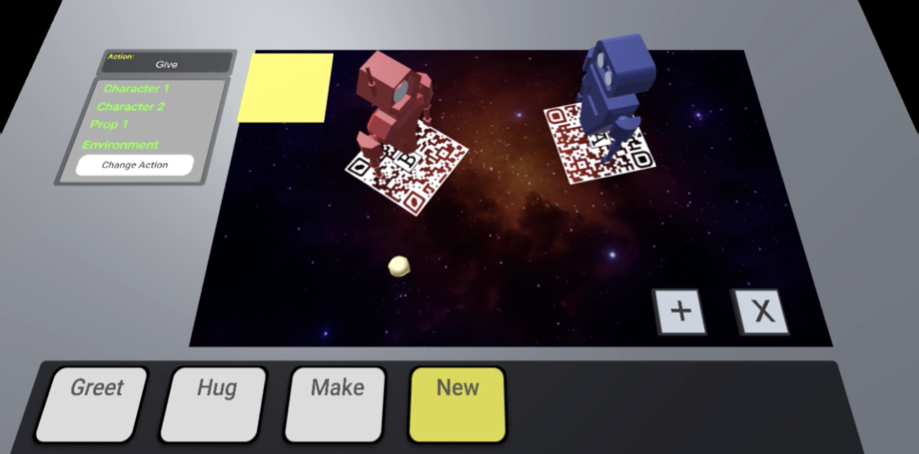
\includegraphics[width=0.75\textwidth]{Figures/Background/tools/M.Kegeleers.png}
    \caption{Content Design Tool Examples - ARtist}
    \label{fig:kelegers}
\end{figure}

\subsection{VR Authoring}
\label{subsec:vr-authoring}
The authoring of \gls{VR} applications is an elaborate and complicated task, requiring resources as time in creating 3D assets and authoring the scene as well as expertise in computer science to program these objects' behaviours throughout the whole experience. An additional difficulty, usually faced when developing applications for \gls{VR}, is the diversity of \gls{VR} hardware setups that need to be configured and maintained \cite{perret_polyvr_2014} but also planned in advance to adapt their characteristics to the development environment.

In our analysis of authoring tools for \gls{VR} systems we decided to adopt the work of Roberto et al.~\cite{marcus_authoring_2016} (\autoref{fig:authoring-tools}) on authoring tools for \gls{AR} to distinguish among programming tools and content design tools.

\subsubsection{Related Works}
\label{subsun:vr-relatedw}
VR development field has been dominated -- for many years -- by game engines based on entity-component architectures, i.e. that allow the definition of virtual objects' behaviours in each frame. These tools such as Unity and Unreal belong, as for \gls{AR} systems, to the class of high-level programming tools and, over the years, many development plugins have been built on top of them to support the diverse multitude of \gls{VR} platforms, namely Google VR SDK, OpenVR SDK, SteamVR SDK and Oculus SDK.
Notwithstanding these proprietary \glspl{SDK} are platform-specific, they require developers' attention in considering different hardware specification within the same family of products \cite{trentsios_comparing_2020}, that is the case of SteamVR SDK and Oculus SDK, while others do not provide simulation capabilities, forcing programmers to physically attach the target devices to the development environment and test the application being built.

In the last years the research in VR development and efforts made in the evolution of the JavaScript language have seen the birth of WebVR \glspl{API}, that allows applications to run on VR devices in their web browsers exploiting the power of WebGL \glspl{API}. This led to the birth of A-Frame, a \gls{VR} framework implemented on top of Three.js library to build VR scenes using the abstraction level of a web designer and the JavaScript technological stack.

As far as concerned a low-level programming approach to \gls{VR} development, many game engines and VR device libraries are developed using the C++ programming language, on which hence some projects put their bases; some examples are the open source projects VRJuggler, OpenSceneGraph and OpenSG, that provide cross-platform deployment capabilities.

High-Level Content Design tools for \gls{VR}, however, allow to abstract from the hardware setups -- and therefore their related APIs -- as well as avoiding to write low-level code for the development of immersive and interactive virtual environments. PolyVR \cite{perret_polyvr_2014} (\autoref{fig:polyvr}) addresses the needs of a flexible and efficient VR hardware management, an authoring tool with a low learning curve for educators and an adaptable solution to support code re-usability. Its \gls{GUI} separates the content creation process from the hardware configuration, while scripting capabilities are enabled by a Python interpreter to design the application logic, without the need to deploy to test it.
\begin{figure}[h]
    \centering
    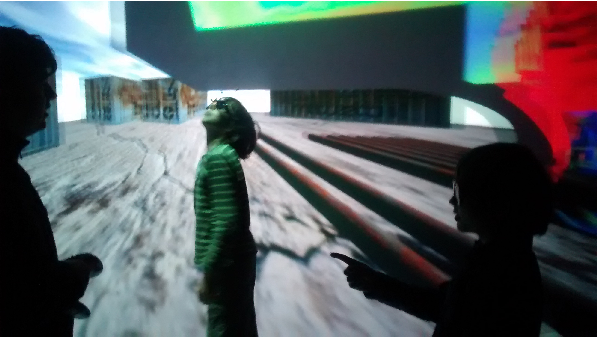
\includegraphics[width=0.75\textwidth]{Figures/Background/tools/polyvr.png}
    \caption{Content Design Tool Examples - PolyVR}
    \label{fig:polyvr}
\end{figure}

Immersive authoring is achieved by FlowMatic \cite{zhang_flowmatic_2020} (\autoref{fig:flowmatic}), whose purpose is to let authors immerse into the same virtual environment they are creating. In their work, Zhang and Oney defined a paradigm based on designer's manipulations of programming primitives to receive an immediate feedback on the designed virtual world. The kind of description this tool complies with is the reactive behaviour specification, i.e. responses to discrete events as user actions or temporal events; other features include the import of 3D models and a \gls{GUI} to program the appearances of objects in a scene. A comparative study with a desktop authoring platform showed that users were able to build interactive VR applications in an immersive authoring environment, considering it intuitive and fun but more importantly helpful in the creation process of this kind of experiences.

\begin{figure}[htbp]
    \centering
    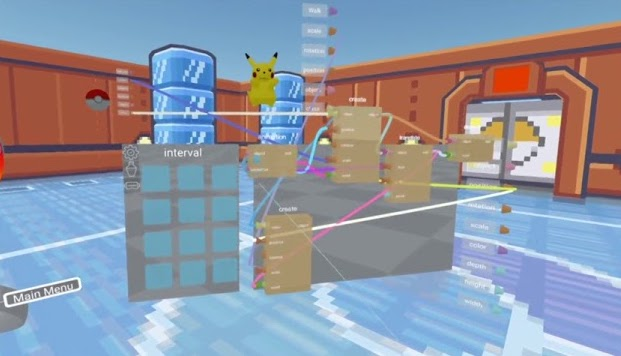
\includegraphics[width=0.75\textwidth]{Figures/Background/tools/flowmatic.jpg}
    \caption{Content Design Tool Examples - FlowMatic}
    \label{fig:flowmatic}
\end{figure}